\documentclass[preview]{standalone}

\usepackage{amsmath}
\usepackage{amssymb}
\usepackage{stellar}
\usepackage{wrapfig}
\usepackage{bettelini}

\hypersetup{
    colorlinks=true,
    linkcolor=black,
    urlcolor=blue,
    pdftitle={Stellar},
    pdfpagemode=FullScreen,
}

\begin{document}

\title{Stellar}
\id{geofisica-europa}
\genpage

\section{Geografia Europea}

\subsection{Regioni}

\includesnpt[width=75\%|src=/snippet/static/europa-regioni.png]{centered-img}

\subsection{Clima}

\begin{snippet}{europa-clima-illustration}
    \setlength{\intextsep}{0pt}%
    \begin{wrapfigure}{l}{.5\textwidth}
        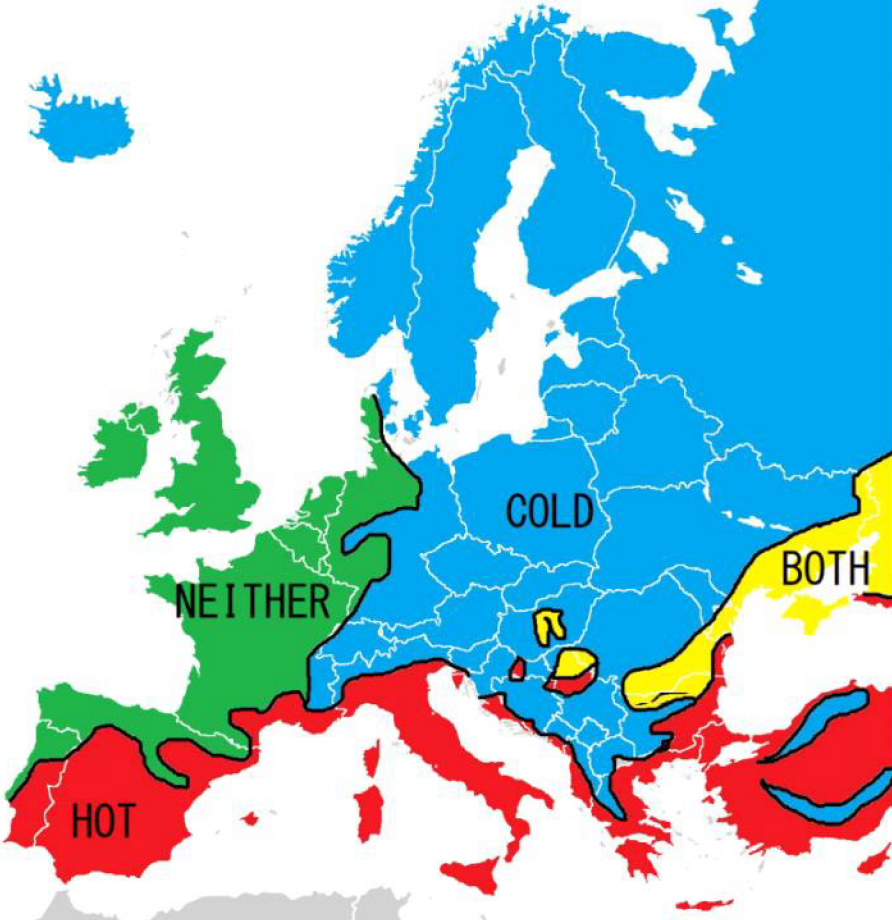
\includegraphics[width=.5\textwidth]{resources/europa-clima.png}
    \end{wrapfigure}
    
    \textbf{Zone climatiche:}
    \begin{itemize}
        \item Calde (HOT): aree influenzate dalla latitudine, che incide
            sull'inclinazione dei raggi solari;
        \item Fredde (COLD): aree con condizioni climatiche fredde, sempre
            influenzate dall'inclinazione dei raggi solari;
        \item Né calde né fredde (NEITHER): aree influenzate dalle correnti del Golfo
            e dalla vicinanza a grandi masse d'acqua;
        \item Entrambe (BOTH): aree che mostrano caratteristiche sia di
            continentalità che di presenza di catene montuose. 
    \end{itemize}
    \wrapfill
\end{snippet}

\end{document}